%!TEX encoding = UTF-8 Unicode
\documentclass[12pt]{article} 
\usepackage[left=0.75in,top=0.7in,right=0.75in,bottom=0.3in]{geometry} % Document margins
\usepackage{CJK}
\usepackage{graphicx}
\usepackage{mathtools}
\usepackage{mathrsfs}
\usepackage{amssymb}
\usepackage{hyperref}
\usepackage{sidecap}
\usepackage{makecell}

\makeatletter
\renewenvironment{itemize}
{\list{$\bullet$}{\leftmargin\z@ \labelwidth\z@ \itemindent-\leftmargin
\let\makelabel\descriptionlabel}}
{\endlist}
\makeatother

\begin{CJK}{UTF8}{bsmi}
\title{\textbf{Homework5 / Test of Generalization}}
\author{\textbf{李豪韋 (HW-Lee) ID 103061527}}
\date{}

\begin{document}
\vspace*{-60pt}
    {\let\newpage\relax\maketitle}

\section*{Overview}
\vspace{-20pt}
\noindent\makebox[\linewidth]{\rule{\textwidth}{0.4pt}}
\vspace{5pt}

This project is followed by the last project: building a  system successfully classifying most of the digits into their own classes. In the process of training, we tried to use any algorithm to make the I/O function close to given data as much as possible. In order to avoid overfitting, we even used cross-validation: separating the dataset into $k$ pieces ($k=8$ in last project) and then hiding one of them as testing data. \\

However, although we used some methodologies to make the system better, it is essential that we need to run a 'REAL' process. As a result, if we call  the last project a 'training stage', this project can be called 'generalization stage', which involves no other algorithm to change the behavior of our system. There are 2000 images given in this project, which consists of two classes of digits (200 images of each class). Optimistically, the accuracy we get with testing data will be close to that with training data. \\

The more detailed information of the code is publicly available on \href{https://github.com/HW-Lee/2015-NN-Homeworks/tree/master/HW05}{$\mathsf{https://github.com/HW}$-$\mathsf{Lee/2015}$-$\mathsf{NN}$-$\mathsf{Homeworks/tree/master/HW05}$}. \\

Recap: The structure I used.

\begin{SCfigure}[][h]
	\hspace*{-2em}
	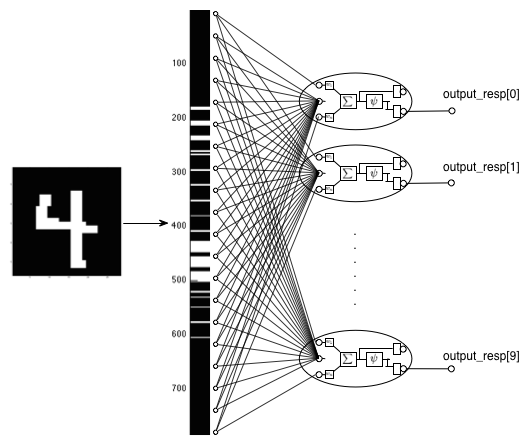
\includegraphics[scale=.65]{../res/netStruct.png}
	\caption{The structure of net. It simply consists of 10 neurons without any hidden unit, which acts like a linear filter, and the image data will be reshaped from 2D to 1D then all pixels will be regarded as an input port. However, the only thing different from the linear filter implemented in Hw2 is that the linear outputs are cascaded to the logistic function that maps any real value into a value ranged from 0 to 1, in order to make the output a measure of 'confidence'. Finally, the prediction is followed by the rule of choosing the class which turns out the highest confidence.}
\end{SCfigure}

\newpage

\section*{Results}
\vspace{-20pt}
\noindent\makebox[\linewidth]{\rule{\textwidth}{0.4pt}}

\begin{enumerate}
	\item Confusion Matrix and False Predicted Averaged Results
	\hspace{-2em}
	\begin{figure}[ht]
	\begin{minipage}[c][11cm][t]{.49\textwidth}
		\centering
		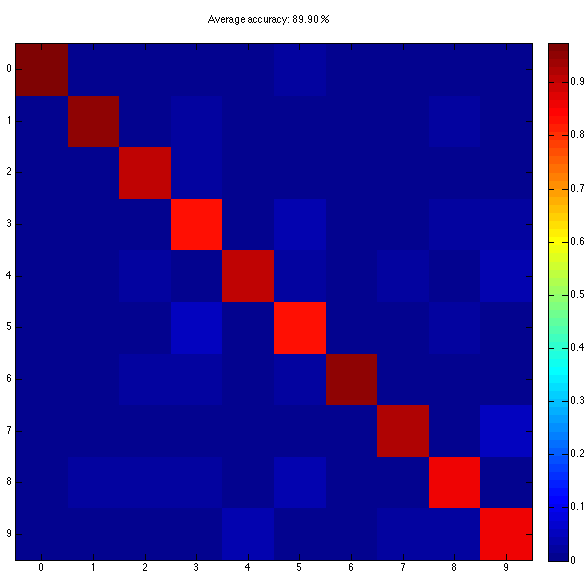
\includegraphics[scale=.5]{../res/confusion.png}
		\vspace{-2.3em}
		\caption{the average accuracy is 0.899}
	\end{minipage}
	\hspace{4em}
	\begin{minipage}[c][11cm][t]{.49\textwidth}
		\vspace{1.8em}
		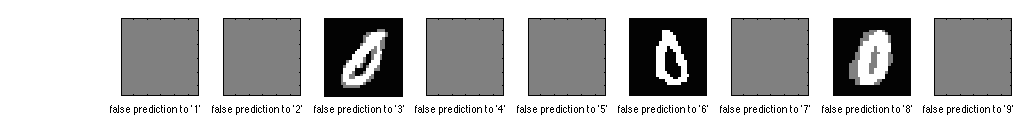
\includegraphics[scale=.2]{../res/fp0.png}
		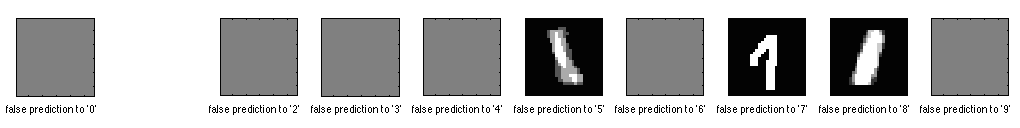
\includegraphics[scale=.2]{../res/fp1.png}
		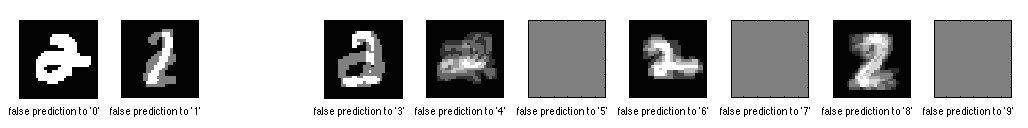
\includegraphics[scale=.2]{../res/fp2.png}
		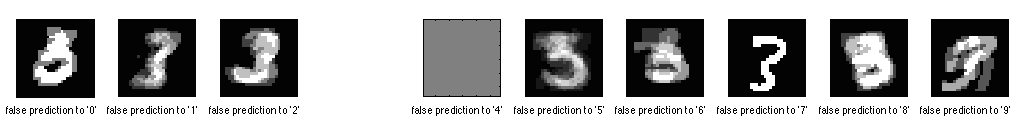
\includegraphics[scale=.2]{../res/fp3.png}
		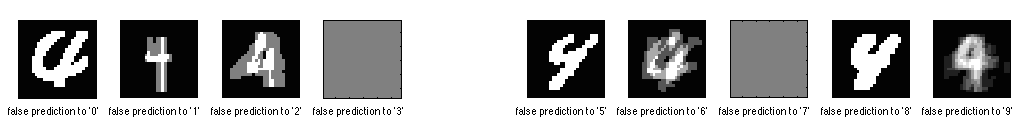
\includegraphics[scale=.2]{../res/fp4.png}
		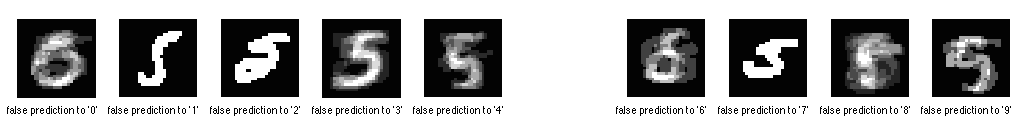
\includegraphics[scale=.2]{../res/fp5.png}
		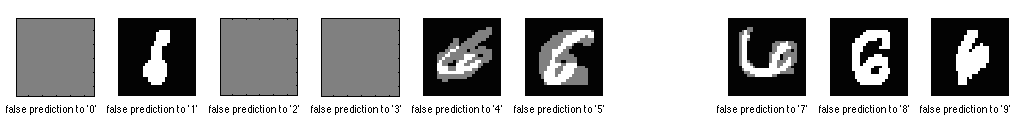
\includegraphics[scale=.2]{../res/fp6.png}
		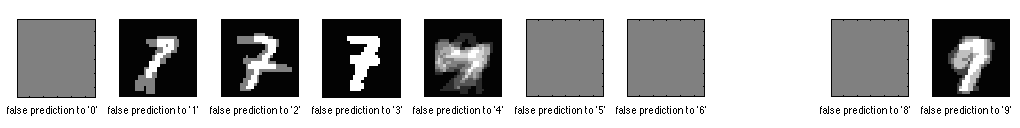
\includegraphics[scale=.2]{../res/fp7.png}
		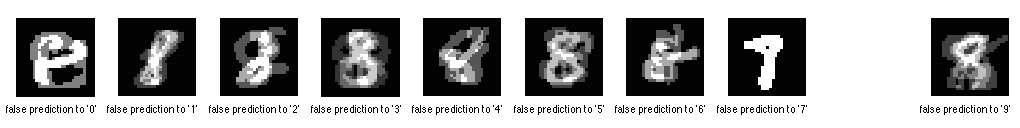
\includegraphics[scale=.2]{../res/fp8.png}
		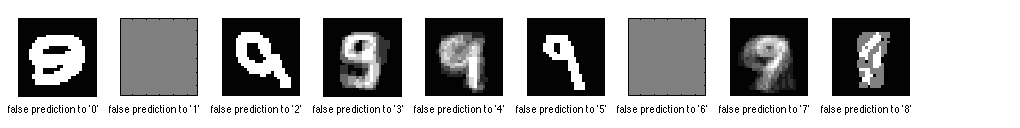
\includegraphics[scale=.2]{../res/fp9.png}
		\vspace{-.5em}
		\hspace{-1em}
		\caption{averaged false predicted images}
	\end{minipage}
	\end{figure}
	\item Averaged Response of each class
	\vspace{-0em}
	\begin{figure}[ht]
		\hspace{-3em}
		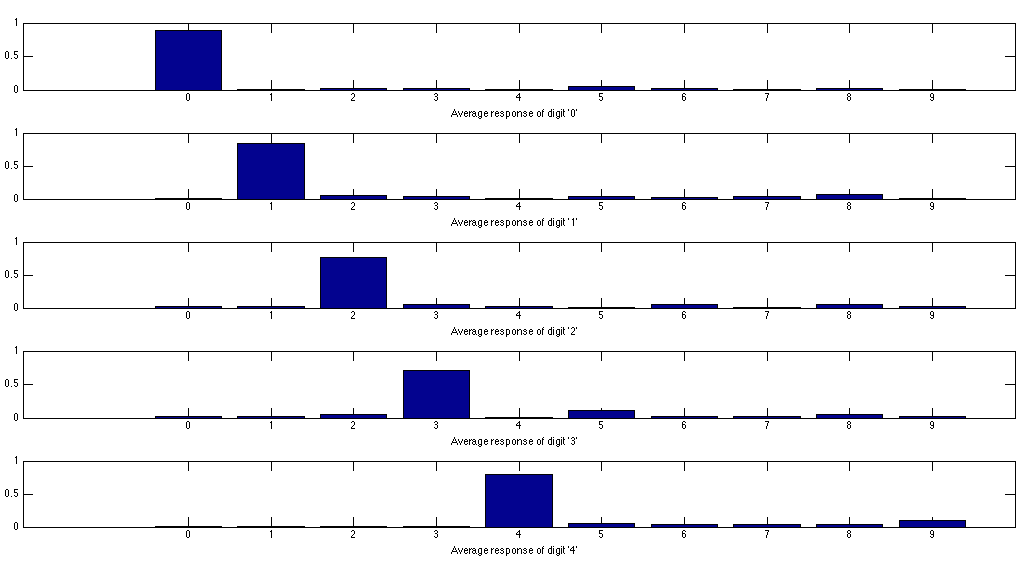
\includegraphics[scale=.28]{../res/resp0-4.png}
		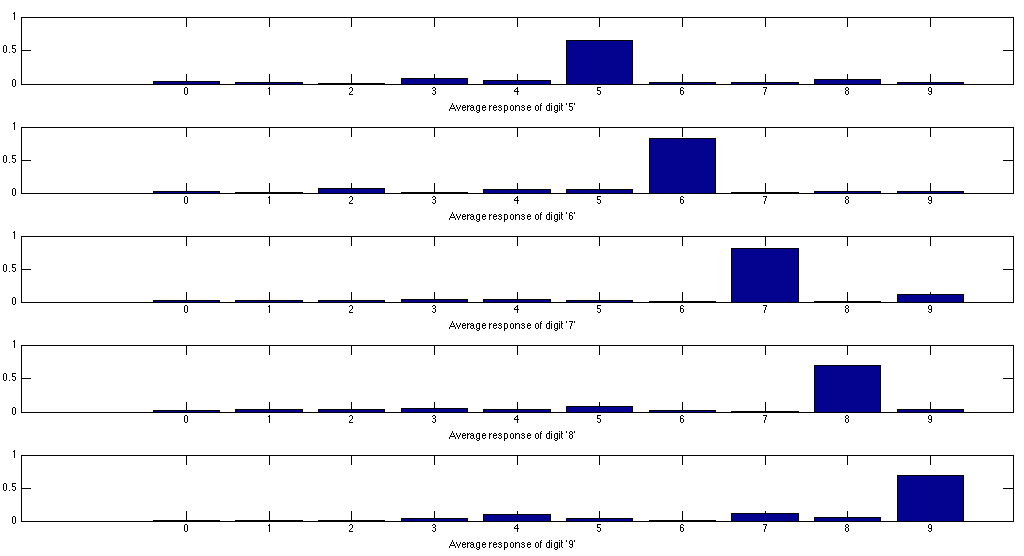
\includegraphics[scale=.28]{../res/resp5-9.png}
		\caption{Averaged Response (left-side: 0-4, and right-side: 5-9, from top to bottom)}
	\end{figure}
	
\end{enumerate}

\newpage
\section*{Discussion}
\vspace{-20pt}
\noindent\makebox[\linewidth]{\rule{\textwidth}{0.4pt}}

\begin{enumerate}
	\item Compare to the accuracy evaluated with cross-validation
	\begin{center}
	\begin{tabular}{|c|c|c|c|c|c|c|c|c|c|c|}
		\hline
		\diaghead{\theadfont Diag ColumnmnHead II}{truth}{result} 
		& '0' & '1' & '2' & '3' & '4' & '5' & '6' & '7' & '8' & '9' \\
		\hline
		'0' & {\bf 0.99} & 0.00 & 0.00 & 0.00 & 0.00 & 0.00 & 0.00 & 0.00 & 0.01 & 0.00 \\ 
		\hline
		'1' & 0.00 & {\bf 0.94} & 0.02 & 0.00 & 0.00 & 0.02 & 0.00 & 0.00 & 0.02 & 0.00 \\ 
		\hline
		'2' & 0.01 & 0.01 & {\bf 0.87} & 0.00 & 0.01 & 0.00 & 0.01 & 0.03 & 0.05 & 0.01 \\ 
		\hline
		'3' & 0.01 & 0.00 & 0.04 & {\bf 0.84} & 0.01 & 0.04 & 0.02 & 0.03 & 0.01 & 0.00 \\ 
		\hline
		'4' & 0.00 & 0.01 & 0.03 & 0.01 & {\bf 0.85} & 0.01 & 0.02 & 0.03 & 0.02 & 0.02 \\ 
		\hline
		'5' & 0.05 & 0.00 & 0.00 & 0.07 & 0.03 & {\bf 0.79} & 0.01 & 0.00 & 0.04 & 0.01 \\ 
		\hline
		'6' & 0.00 & 0.00 & 0.00 & 0.01 & 0.01 & 0.03 & {\bf 0.94} & 0.00 & 0.01 & 0.00 \\ 
		\hline
		'7' & 0.01 & 0.01 & 0.01 & 0.00 & 0.01 & 0.00 & 0.00 & {\bf 0.93} & 0.00 & 0.03 \\ 
		\hline
		'8' & 0.01 & 0.03 & 0.01 & 0.04 & 0.01 & 0.00 & 0.01 & 0.02 & {\bf 0.85} & 0.02 \\ 
		\hline
		'9' & 0.04 & 0.02 & 0.01 & 0.02 & 0.06 & 0.02 & 0.01 & 0.04 & 0.01 & {\bf 0.77} \\ 
		\hline
	\end{tabular}
	\end{center}

	\hspace{-3em}
	\begin{tabular}{|c|c|c|c|c|c|c|c|c|c|c|}
		\hline
		\diaghead{\theadfont Diag ColumnmnHead II}{truth}{result} 
		& '0' & '1' & '2' & '3' & '4' & '5' & '6' & '7' & '8' & '9' \\
		\hline
		'0' & {\bf 0.975} & 0.000 & 0.000 & 0.010 & 0.000 & 0.000 & 0.005 & 0.000 & 0.010 & 0.000 \\ 
 		\hline 
		'1' & 0.000 & {\bf 0.955} & 0.000 & 0.000 & 0.000 & 0.015 & 0.000 & 0.005 & 0.025 & 0.000 \\ 
 		\hline 
		'2' & 0.005 & 0.010 & {\bf 0.900} & 0.010 & 0.025 & 0.000 & 0.020 & 0.000 & 0.030 & 0.000 \\ 
 		\hline 
		'3' & 0.010 & 0.025 & 0.020 & {\bf 0.825} & 0.000 & 0.055 & 0.025 & 0.005 & 0.020 & 0.015 \\ 
 		\hline 
		'4' & 0.005 & 0.010 & 0.010 & 0.000 & {\bf 0.910} & 0.005 & 0.015 & 0.000 & 0.005 & 0.040 \\ 
		 \hline 
		'5' & 0.025 & 0.005 & 0.005 & 0.035 & 0.030 & {\bf 0.825} & 0.020 & 0.005 & 0.035 & 0.015 \\ 
		 \hline 
		'6' & 0.000 & 0.005 & 0.000 & 0.000 & 0.010 & 0.010 & {\bf 0.955} & 0.010 & 0.005 & 0.005 \\ 
 		\hline 
		'7' & 0.000 & 0.010 & 0.010 & 0.005 & 0.030 & 0.000 & 0.000 & {\bf 0.925} & 0.000 & 0.020 \\ 
 		\hline 
		'8' & 0.010 & 0.020 & 0.015 & 0.025 & 0.015 & 0.020 & 0.015 & 0.005 & {\bf 0.855} & 0.020 \\ 
 		\hline 
		'9' & 0.005 & 0.000 & 0.005 & 0.025 & 0.035 & 0.005 & 0.000 & 0.050 & 0.010 & {\bf 0.865} \\ 
 		\hline 
	\end{tabular}

	\begin{flushleft}
		The result shows that 1) the system is neither overfitting nor underfitting, 2) the simple structure is sufficiently complex to learn the task.	
	\end{flushleft}		
	
	\item Is deep learning, which contains more than 3 layers, needed to learn this task?
	\begin{flushleft}
		The answer is no, I think, because 1) the dataset is well-preprocessed: the digits have roughly same size, the skewness can be roughly ignored... 2) the dataset has been binarized, which significantly decreases the variance of outputs space. In addition, convolutional neural network might be able to increase the accuracy, but might cause overfitting issue or multiple elements activate with same features issue.
	\end{flushleft}
	
	\item Are wrongly predicted results really difficult to be recognized?
	\begin{flushleft}
		Actually it is not difficult. The reason why the system misclassifies these instances might be that the training dataset is too small to make the system figure out the most critical features of each class, and the accuracy will be lifted after increasing the number of training instances.
	\end{flushleft}
	
\end{enumerate}

\end{CJK}
\end{document}